% !TeX root = main.tex
\chapter*{INTRODUCCIÓN}
\addcontentsline{toc}{chapter}{INTRODUCCIÓN}
\setcounter{chapter}{1}

\section{OBJETIVO GENERAL}
Implementar un enlace vehículo a infraestructura (V2I) basado en la capa física del estándar IEEE 802.11bb dentro del espectro de la luz visible VLC con una de simulación en Python, con el fin de analizar estadísticamente el impacto de condiciones climáticas adversas sobre la confiabilidad y el desempeño del enlace óptico en entornos urbanos en términos de BER, SNR y tasa efectiva de transmisión.

\section{OBJETIVOS ESPECÍFICOS}
\begin{enumerate}
	\item Desarrollar la fundamentación teórica y matemática del transmisor-receptor basado en la capa física del estándar IEEE 802.11bb.
	\item Diseñar y programar en Python el motor de simulación de la capa física, incluyendo las etapas de transmisión y recepción conectadas por el canal óptico.
	\item Evaluar el desempeño del canal óptico-vehicular mediante su comparación con un canal equivalente AWGN, desarrollando simulaciones en condiciones climáticas propias de entornos urbanos y presentando los resultados en términos de BER versus SNR y velocidad efectiva de transmisión, con el fin de verificar la coherencia entre los resultados numéricos y el comportamiento teórico esperado del enlace.
\end{enumerate}

\section{ALCANCE}
El presente Trabajo de Integración Curricular contempla el diseño, implementación y evaluación de un modelo de simulación de un sistema de comunicación vehicular óptica en un enlace vehículo a infraestructura (V2I) y fundamentado en los principios técnicos del estándar IEEE 802.11bb. El estudio se desarrollará a nivel de capa física, considerando un enlace óptico inalámbrico en línea de vista (LOS).

En la fase de diseño se establecerá la fundamentación teórica y matemática de los bloques que conforman el sistema de comunicación a simular, incluyendo transmisor-receptor y el canal óptico-vehicular. Se definirá el modelo de generación de bits, codificación FEC, modulación digital y procesamiento OFDM (asignación de subportadoras, IFFT e inserción de prefijo cíclico), junto con la adaptación de la señal al esquema de modulación en intensidad y detección directa mediante la adición de un bias DC y el modelado de la conversión eléctrica-óptica del LED considerando su respuesta en frecuencia y posibles no linealidades. Se diseñará el modelo del canal óptico VLC en línea de vista (LOS) con patrón de radiación Lambertiano, parámetros geométricos del enlace y fuentes de ruido óptico. Se establecerá el modelo del receptor incluyendo el fotodetector con su responsividad y la cadena de procesamiento inversa compuesta por remoción de prefijo cíclico, FFT, demapping de constelación, demodulación y decodificación, permitiendo la recuperación de los bits transmitidos y la evaluación analítica del desempeño del sistema.


En la fase de implementación se desarrollará en Python el motor de simulación que integrará los bloques de transmisión, canal óptico y recepción dentro de una misma cadena funcional. Posteriormente, el sistema se someterá a una evaluación bajo un canal equivalente AWGN, comparando los resultados obtenidos con el comportamiento teórico esperado y presentando métricas en términos de BER versus SNR y velocidad efectiva de transmisión, con el propósito de verificar la coherencia del modelo en condiciones controladas antes de analizar escenarios atmosféricos propios del entorno urbano.

En la fase de pruebas, evaluación y análisis, se ejecutarán simulaciones mediante el método de Montecarlo para analizar el desempeño del sistema bajo diferentes condiciones climáticas. Se estimarán métricas como la tasa de error de bit (BER), la relación señal a ruido (SNR) y la tasa efectiva de transmisión.

El alcance se limita al análisis mediante simulación computacional y no contempla implementación experimental en hardware ni validación en entornos reales.

\section{MARCO TEÓRICO}
En la era de los Sistemas Inteligentes de Transporte (ITS, \textit{Intelligent Transportation Systems}) y la conducción autónoma, la comunicación vehicular V2X (\textit{Vehicle-to-Everything}) es parte importante para garantizar la seguridad vial, la eficiencia del tráfico y la coordinación en tiempo real entre vehículos, infraestructuras y usuarios. Tradicionalmente, las tecnologías basadas en radiofrecuencia (RF) como DSRC (\textit{Dedicated Short-Range Communications}) basada en IEEE 802.11p y C-V2X (\textit{Cellular Vehicle-to-Everything}) basada en estándares celulares LTE/5G han impulsado estos avances. Sin embargo estas tecnologías enfrentan limitaciones en entornos urbanos congestionados, como el espectro saturado, la interferencia electromagnética y la latencia en escenarios de alta densidad \cite{feukeu2023enhancing}.

Por esa razón, la Comunicación por Luz Visible (VLC) surge como una alternativa complementaria, al aprovechar la infraestructura de iluminación LED ya existente en faros, luces traseras y semáforos para transmitir datos a través del espectro visible. VLC tiene la gran ventaja de ocupar una porción del espectro electromagnético que no requiere licencias, está subexplotado, tiene inmunidad a interferencias de RF y una mayor seguridad física del enlace \cite{georlette2020visible}.


 

\subsection{COMUNICACIÓN VEHICULAR Y PRINCIPIOS DE LOS SISTEMAS VLC}
La comunicación vehicular consiste en el intercambio de información entre vehículos con el objetivo de optimizar la seguridad, reducir congestiones y dar soporte a la conducción autónoma. Para esta aplicación, la Comunicación por Luz Visible (VLC) se presenta como una tecnología de comunicación óptica inalámbrica que utiliza el espectro de luz visible ---e incluso bandas cercanas al infrarrojo---  para transmitir datos modulando la intensidad de la luz emitida por LEDs \cite{feukeu2023enhancing, georlette2020visible}.

\subsubsection{Arquitectura de comunicación vehicular V2X y el entorno V2I}
La comunicación V2X cuenta con distintos modos de intercambio de información en función de los actores involucrados como: Comunicación Vehículo a Vehículo (V2V, \textit{Vehicle-to-Vehicle}) para la seguridad cooperativa entre automóviles; Comunicación Vehículo a Infraestructura (V2I) para la interacción con elementos viales; Comunicación Vehículo a Peatón (V2P, \textit{Vehicle-to-Pedestrian}) orientada a la protección de usuarios vulnerables; y Comunicación Vehículo a Red (V2N, \textit{Vehicle-to-Network}) para la conexión con servicios en la nube. En conjunto de actores crea un sistema integral para los ITS porque habilitan el intercambio de datos en tiempo real \cite{feukeu2023enhancing}.

\begin{figure}[htbp]
	\centering
	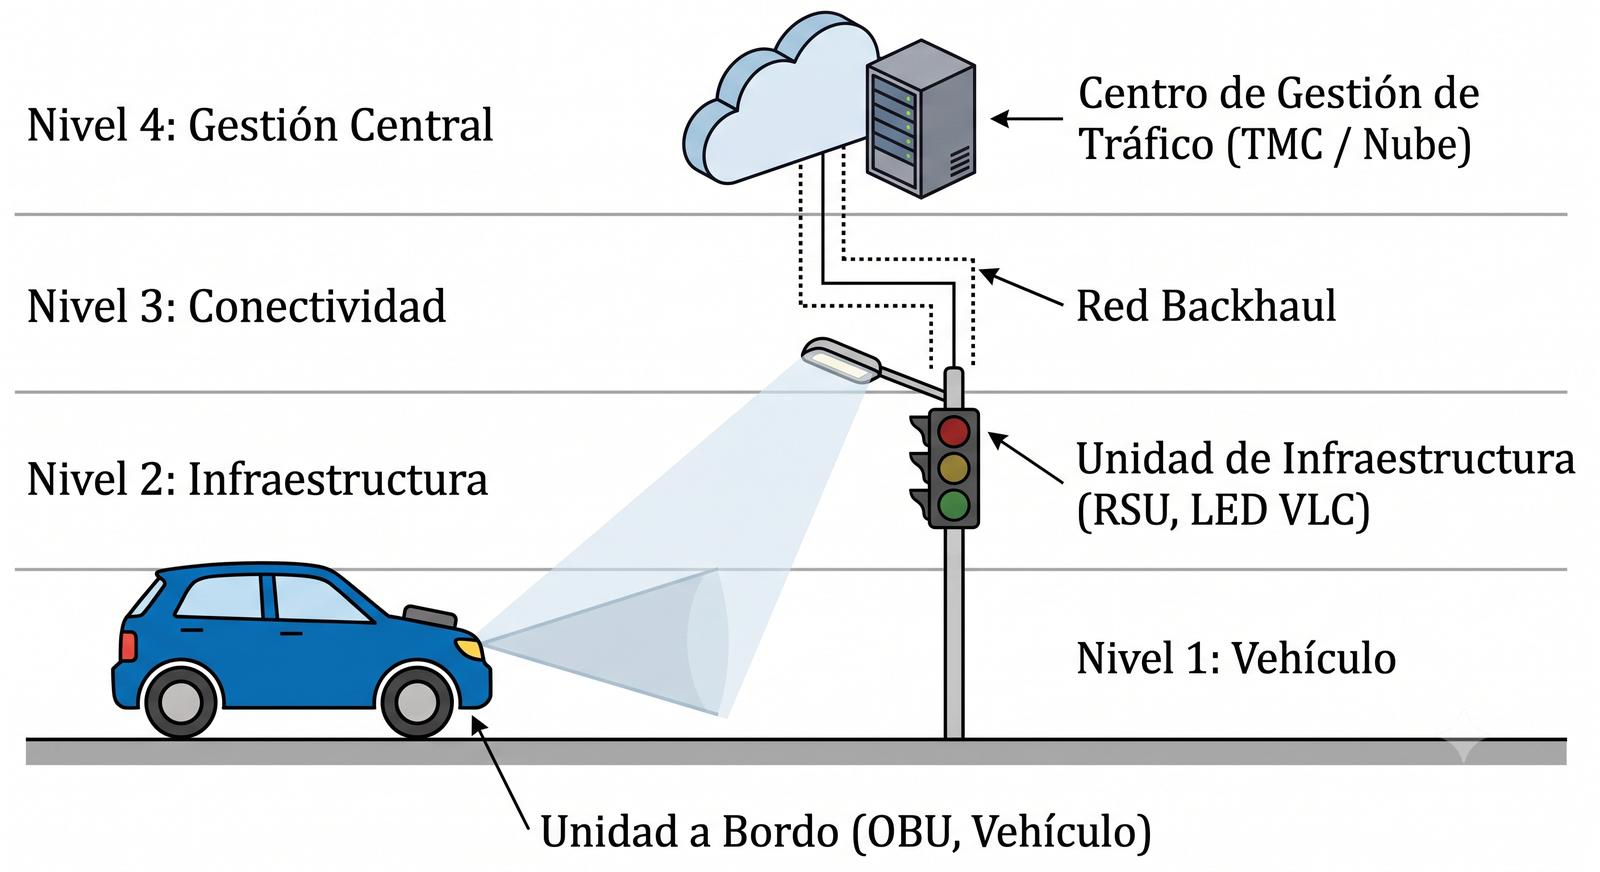
\includegraphics[width=0.9\textwidth]{arquitectura_v2i.png}
	\caption{Arquitectura jerárquica y funcional de un sistema de comunicación V2I basado en VLC.}
	\label{fig:arquitectura_v2i}
\end{figure}

La arquitectura jerárquica del sistema V2I se compone de cuatro niveles estructurados de forma secuencial, tal como se ilustra en la Fig. \ref{fig:arquitectura_v2i}. En el extremo móvil (Nivel 1) se encuentra la Unidad a Bordo (OBU, \textit{On-Board Unit}), encargada de la adquisición de telemetría vehicular mediante los sistemas de diagnóstico internos del automóvil \cite{ieee1609architecture}. Esta interactúa directamente con la Unidad en la Vía (RSU, \textit{Roadside Unit}) ubicada en el Nivel 2, la cual, en entornos de comunicación óptica inalámbrica, adapta las luminarias y la infraestructura vial preexistente en puntos de acceso de datos de alta velocidad \cite{uysal2015vlc}. A su vez, las RSU se interconectan mediante una red de transporte (\textit{backhaul}) en el Nivel 3, encargada de canalizar el flujo de información agregado hacia el Centro de Gestión de Tráfico (TMC, \textit{Traffic Management Center}) o servidores en la nube ubicados en el Nivel 4; en este último nivel jerárquico se ejecutan los algoritmos de procesamiento centralizado y análisis masivo de datos para la optimización del tráfico y la gestión automatizada de la seguridad vial \cite{arena2019overview}.



\subsubsection{Principios fundamentales de los sistemas VLC}
Un sistema VLC opera en la banda de la luz visible, por lo general comprendida entre los 400~nm y 750~nm. Como se ilustra en el diagrama de bloques de la Fig. \ref{fig:bloques_vlc}, la arquitectura de la capa física se compone de tres bloques: Transmisor, canal óptico y receptor. VLC utiliza el principio de modulación de intensidad y detección directa (IM/DD, \textit{Intensity Modulation / Direct Detection}),esta modulación codifica la información variando la potencia óptica instantánea sin modificar su fase ni su frecuencia \cite{georlette2020visible}.

\begin{figure}[htbp]
	\centering
	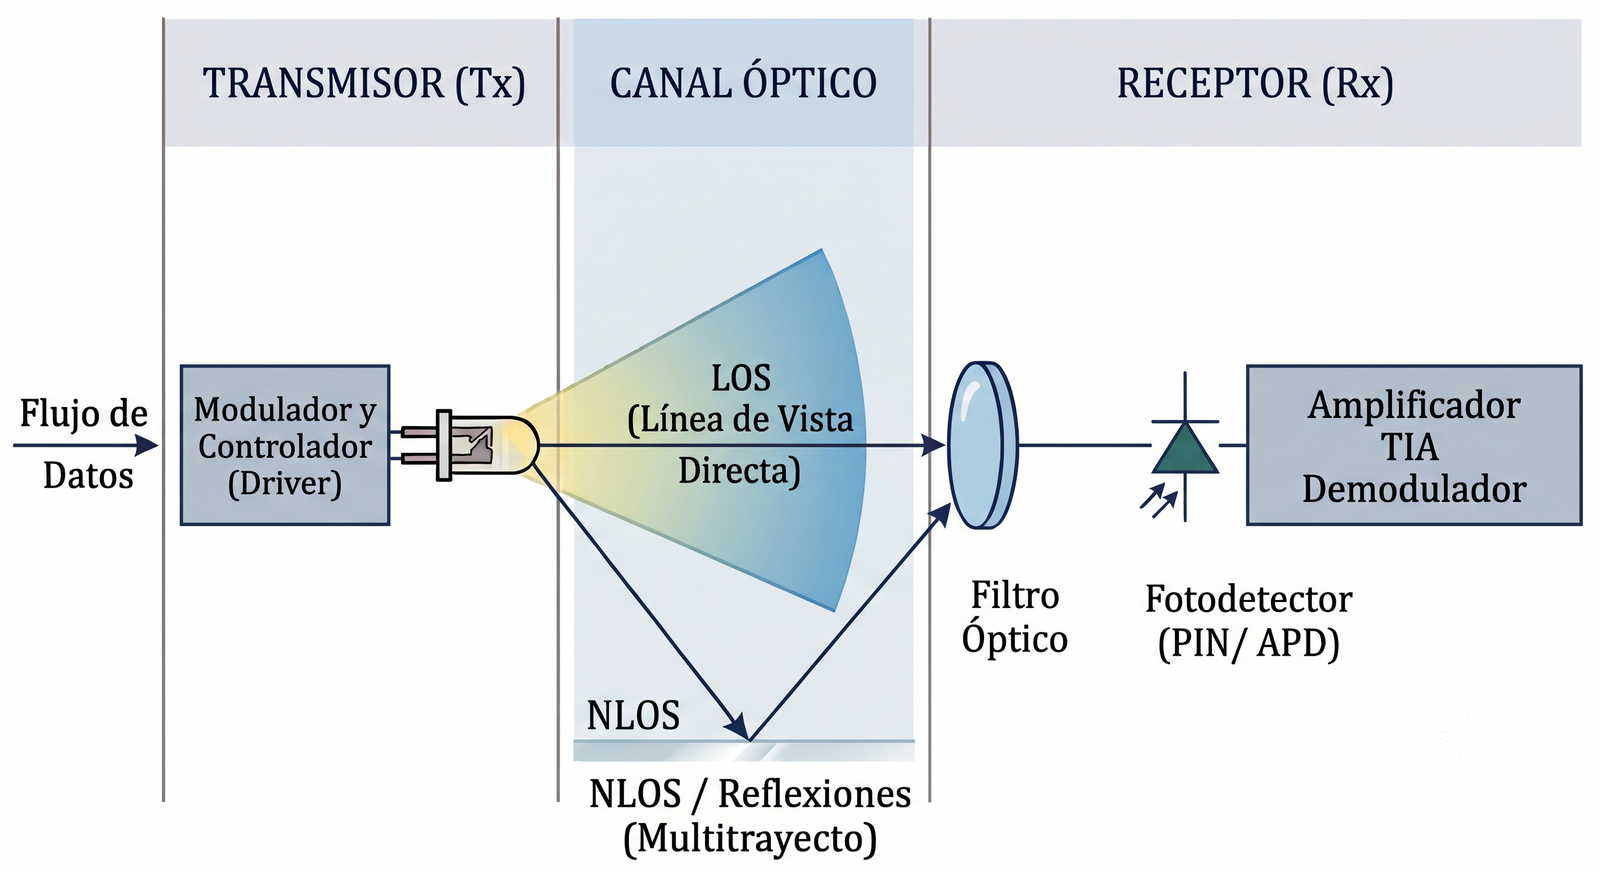
\includegraphics[width=0.85\textwidth]{bloques_vlc.png}
	\caption{Diagrama de bloques de un sistema de comunicación por luz visible (VLC).}
	\label{fig:bloques_vlc}
\end{figure}

El \textbf{bloque transmisor (Tx)} realiza la conversión electroóptica bajo el principio de modulación de intensidad. En esta etapa, los datos digitales son procesados por un modulador y acoplados mediante un circuito de polarización (\textit{driver}) a un diodo emisor de luz (LED), que funciona como el transductor óptico alterando la potencia óptica instantánea de su flujo luminoso, que para no perder el propósito principal de los dispositivos de iluminación trabaja a velocidades imperceptibles para el ojo humano, manteniendo fijas la fase y la frecuencia de la onda electromagnética \cite{ghassemlooy2019optical}.

El \textbf{bloque del canal óptico} es el medio de propagación inalámbrico donde se desplazan los fotones cuya intensidad ha sido modulada. Este bloque determina la atenuación geométrica del enlace y se compone del trayecto directo de línea de vista (LOS) y de las reflexiones secundarias en las superficies del entorno (NLOS, \textit{Non-Line-of-Sight}); el comportamiento de propagación multitrayecto se modela matemáticamente mediante la respuesta al impulso del canal para caracterizar la distorsión y la dispersión temporal de la potencia óptica incidente \cite{uysal2016optical}.

El \textbf{bloque receptor (Rx)} ejecuta la etapa de detección directa para llevar a cabo la conversión optoelectrónica y recuperar la información. Los fotones incidentes pasan por filtros ópticos y concentradores que delimitan el campo de visión (FOV, \textit{Field of View}), incidiendo directamente sobre un fotodetector (fotodiodo PIN, \textit{Positive-Intrinsic-Negative}, o APD, \textit{Avalanche Photodiode}). Este transductor genera una corriente eléctrica proporcional a la potencia óptica capturada, permitiendo que un amplificador de transimpedancia (TIA, \textit{Transimpedance Amplifier}) eleve el nivel de la señal para finalmente demodularla \cite{elgala2011indoor}.




\subsection{ESTÁNDAR IEEE 802.11BB}

El estándar IEEE 802.11bb (\textit{Amendment 6: Light Communications}) \cite{ieee80211bb2023} define las directrices para la integración de las comunicaciones ópticas en entornos inalámbricos, facilitando su aplicación en redes vehiculares. Esta enmienda al estándar base IEEE 802.11 especifica las modificaciones requeridas en las capas física (PHY, \textit{Physical Layer}) y de control de acceso al medio (MAC, \textit{Medium Access Control}) para dar soporte a los enlaces ópticos, garantizando la coexistencia e interoperabilidad con las redes inalámbricas de radiofrecuencia convencionales. Bajo este principio, se viabiliza el uso de los sistemas de iluminación vehicular como puntos de acceso de datos.

Los protocolos de este estándar se organizan en una estructura jerárquica que separa las funciones lógicas de los procesos dependientes del medio físico. En el nivel superior, la capa MAC gestiona el direccionamiento, la seguridad y el acceso compartido al medio óptico. Inmediatamente debajo, la capa PHY se encarga de la transmisión efectiva de bits sobre el canal. Para maximizar el aprovechamiento del ancho de banda, el estándar adopta los mecanismos de alta eficiencia (HE, \textit{High Efficiency}) heredados de la enmienda IEEE 802.11ax, reconfigurándolos bajo la especificación HE-LC (\textit{High Efficiency Light Communications}) para el procesamiento de señales mediante multiplexación por división de frecuencias ortogonales (OFDM, \textit{Orthogonal Frequency Division Multiplexing}) adaptada a canales ópticos \cite{obeed2019optimize}.

Esta base normativa permite que el sistema soporte diversas tasas de transferencia y niveles de robustez, adaptándose de forma dinámica a las condiciones cambiantes del canal vehicular V2I mediante el uso de esquemas de modulación adaptativos.

\subsubsection{Modos de operación}
El estándar IEEE 802.11bb permite la coexistencia de diferentes perfiles en la capa física, asegurando que los dispositivos establezcan enlaces ópticos de acuerdo con sus capacidades de hardware. Estos niveles se segmentan en capacidades de rendimiento heredadas (\textit{Legacy Non-HT}) y capacidades de alta eficiencia (HE, \textit{High Efficiency}). Mientras que los modos heredados se limitan a garantizar la compatibilidad operativa básica mediante transmisiones de portadora única o esquemas OFDM convencionales, el modo HE define perfiles optimizados para canales de 20~MHz mediante la reconfiguración de la subcapa física \cite{ieee80211bb2023}. 

El modo HE implementa una reducción a la cuarta parte en el espaciamiento entre subportadoras ortogonales ($\Delta f = 78.125$~kHz), lo que resulta en una duración del símbolo OFDM útil cuatro veces mayor ($12.8~\mu$s) en comparación con las arquitecturas previas \cite{ieee80211bb2023}. Desde la perspectiva del canal físico, esta ampliación temporal del símbolo, combinada con la inserción de intervalos de guarda extendidos, proporciona inmunidad estricta frente a la interferencia entre símbolos (ISI, \textit{Inter-Symbol Interference}) inducida por la dispersión por retraso multitrayecto (\textit{multipath delay spread}) característica del asfalto y el entorno urbano, mitigando el desvanecimiento selectivo en frecuencia provocado por la alta movilidad V2I \cite{luo2017vlc}.

El modo de alta eficiencia utiliza multiplexación por división de frecuencias ortogonales (OFDM) para el enlace de datos. El canal de 20~MHz se organiza en un bloque unificado de subportadoras que son ocupadas en su totalidad por la Unidad a Bordo (OBU) vehicular durante cada ranura de transmisión, optimizando la densidad de potencia espectral en el enlace de subida hacia la Unidad en la Vía (RSU) \cite{feukeu2023enhancing}.


\subsubsection{Arquitectura de la capa de control de acceso al medio MAC}
La capa MAC en el estándar IEEE 802.11bb es la responsable de organizar los datos del usuario en estructuras lógicas, gestionar el direccionamiento y coordinar el acceso compartido al medio óptico inalámbrico. La unidad fundamental de procesamiento en este nivel es la Unidad de Datos de Protocolo MAC (MPDU, \textit{MAC Protocol Data Unit}). Esta estructura encapsula la carga útil proveniente de las aplicaciones vehiculares y añade un encabezado de control indispensable para garantizar que el mensaje sea direccionado correctamente y se transmita libre de errores dentro del entorno V2I. Las secciones principales que componen esta trama se detallan en la Tabla \ref{tab:mpdu}.

\begin{table}[htbp]
	\centering
	\caption{Componentes de la Trama MPDU según el Estándar IEEE 802.11.}
	\label{tab:mpdu}
	\begin{tabular}{|p{3.5cm}|p{10.5cm}|}
		\hline
		\textbf{Parte de la MPDU} & \textbf{Descripción y Funciones} \\ \hline
		Encabezado MAC & Contiene el control de trama, duración, direcciones de destino/origen y control de secuencia. \\ \hline
		Cuerpo de la Trama & Aloja la carga útil (\textit{payload}) con la información de la aplicación o capas superiores. \\ \hline
		Secuencia de Verificación (FCS) & Secuencia de verificación de trama mediante CRC de 32~bits para detección de errores. \\ \hline
	\end{tabular}
\end{table}

El campo FCS utiliza un algoritmo de redundancia cíclica para que el receptor valide la integridad de los datos y descarte de forma inmediata los paquetes que hayan sufrido alteraciones debido al ruido intrínseco del canal \cite{ieee80211bb2023}. Para maximizar el aprovechamiento del canal en escenarios de alta densidad y movilidad vehicular, la capa MAC implementa la agregación de tramas (A-MPDU). Esta técnica consiste en agrupar múltiples unidades MPDU en una sola transmisión física, lo que reduce el impacto del tiempo de espera entre tramas (\textit{interframe spacing}) y disminuye drásticamente la sobrecarga de señalización, permitiendo el envío constante de alertas de seguridad vial con una latencia mínima \cite{georlette2020visible}.



Además de la estructuración de datos, la función crítica de la capa MAC radica en la administración del acceso múltiple mediante el protocolo CSMA/CA (\textit{Carrier Sense Multiple Access with Collision Avoidance}). Para coordinar las transmisiones vehiculares distribuidas y evitar colisiones destructivas en el espectro óptico, la capa MAC explota las indicaciones lógicas del mecanismo de Evaluación de Canal Libre (CCA, \textit{Clear Channel Assessment}) provistas por la capa física \cite{solaija2023light}. 

Este mecanismo de gestión opera bajo dos métodos concurrentes administrados por la lógica MAC. El primero es la detección de energía (ED), que determina el estado de ocupación del canal basándose en los umbrales de potencia óptica total medidos en el receptor para identificar fuentes de luz ambientales o interferencias secundarias \cite{ieee80211bb2023}. El segundo es la detección de portadora (CS), encargado de reconocer la estructura de preámbulo específica de una trama legítima del estándar. La integración de estos procesos le permite a la capa MAC discernir de forma precisa el estado del medio de transmisión, gobernando los tiempos de acceso y los algoritmos de respaldo (*backoff*) indispensables para mitigar la congestión en redes V2I de alta concurrencia \cite{feukeu2023enhancing}.


\subsubsection{Arquitectura de la capa física PHY}
La capa física (PHY) del estándar IEEE 802.11bb es la responsable de la transmisión efectiva de los bits sobre el medio óptico inalámbrico. Para independizar las funciones de procesamiento lógicas de las restricciones del hardware de transmisión-recepción, esta capa se subdivide en dos subcapas principales: el Procedimiento de Convergencia de la Capa Física (PLCP, \textit{Physical Layer Convergence Procedure}) y la subcapa Dependiente del Medio Físico (PMD, \textit{Physical Medium Dependent}) \cite{ieee80211bb2023}. La Tabla \ref{tab:capa_fisica_div} resume la distribución de tareas y la jerarquía funcional de esta arquitectura.

\begin{table}[htbp]
	\centering
	\caption{División Funcional de la Capa Física en el Estándar IEEE 802.11bb.}
	\label{tab:capa_fisica_div}
	\begin{tabular}{|p{3.5cm}|p{4.5cm}|p{6.5cm}|}
		\hline
		\textbf{Subcapa} & \textbf{Función Principal} & \textbf{Descripción Técnica} \\ \hline
		PLCP & Convergencia lógicas & Prepara la MPDU añadiendo preámbulos y gestiona la asignación de símbolos OFDM. \\ \hline
		PMD & Interfaz con el medio & Realiza la conversión electroóptica (Tx) y la conversión optoelectrónica (Rx). \\ \hline
	\end{tabular}
\end{table}

La subcapa PLCP funciona como un adaptador entre la capa MAC y el medio físico. Tomando la MPDU provista por la capa superior, le añade un preámbulo y un encabezado físico para formar la Unidad de Datos de Protocolo de la Capa Física (PPDU, \textit{PHY Protocol Data Unit}) \cite{kim2022ieee}. Esta subcapa gestiona la asignación de los bits en símbolos OFDM y organiza la estructura de la trama que permite al receptor sincronizarse correctamente, siguiendo los lineamientos de la Cláusula 33.2.1 del estándar \cite{ieee80211bb2023}. Por su parte, la subcapa PMD es la responsable de la transmisión real de los bits sobre el canal óptico, definiendo los parámetros de modulación de intensidad y detección directa de la unidad Tx/Rx sin alterar la lógica de comunicación superior.

\paragraph{Descripción detallada de los bloques del transmisor-receptor}
El sistema transmisor-receptor basado en la enmienda \cite{ieee80211bb2023} opera mediante una arquitectura simétrica de procesamiento de señal donde cada etapa del bloque transmisor posee una función inversa homóloga dentro del bloque receptor. Esta topología asegura que la unidad PPDU se adapte a las restricciones físicas del canal óptico e inalámbrico y pueda ser recuperada con una mínima tasa de error en el destino. Los diagramas de flujo y la secuencia del procesamiento para el transmisor y el receptor de la capa física de comunicaciones por luz (LC PHY) se ilustran de forma didáctica en la Fig. \ref{fig:transmisor_bloques} y la Fig. \ref{fig:receptor_bloques}, respectivamente.

\begin{figure}[htbp]
	\centering
	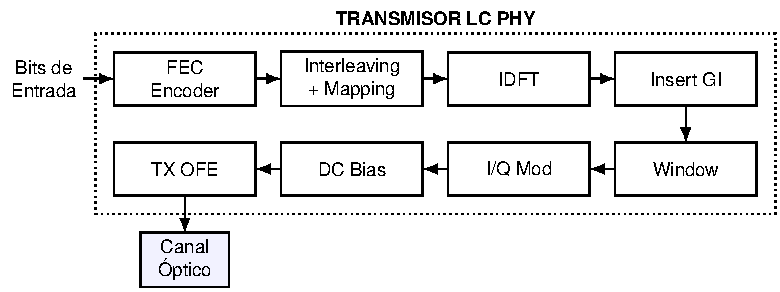
\includegraphics{fig_transmisor_bloques}
	\caption{Diagrama de bloques del transmisor de la capa física (LC PHY).}
	\label{fig:transmisor_bloques}
\end{figure}

\begin{figure}[htbp]
	\centering
	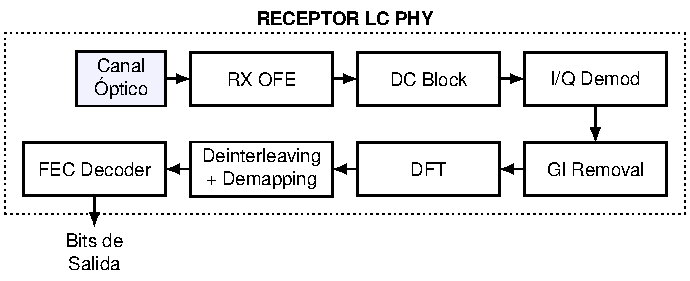
\includegraphics{fig_receptor_bloques}
	\caption{Diagrama de bloques del receptor de la capa física (LC PHY). }
	\label{fig:receptor_bloques}
\end{figure}

A partir de la correspondencia visual establecida entre ambas cadenas de procesamiento, el comportamiento específico de cada etapa analógica y digital del sistema Tx/Rx se detalla formalmente a continuación:

% ==============================================================================
% NOTA: PEGA AQUÍ TU TEXTO CON LA DESCRIPCIÓN DETALLADA DE CADA BLOQUE FUNCIONAL
En este apartado se describen los procesos técnicos que ejecutan los componentes de la capa física (PHY) del estándar IEEE 802.11bb, analizando su función en la adecuación de la señal para el canal vehicular.

\paragraph{FEC Encoder / Decoder}
El bloque FEC Encoder introduce redundancia estructural y controlada en la secuencia de bits de datos con el objetivo de permitir que el receptor detecte y corrija errores de bit sin requerir retransmisiones. Aunque la normativa IEEE 802.11bb define códigos LDPC (\textit{Low-Density Parity-Check}) para la enmienda HE-LC \cite{ieee80211bb2023}, con fines de viabilidad y eficiencia computacional en las simulaciones de esta tesis se implementa un codificador convolucional de tasa de codificación base $R_c = 1/2$ y una longitud de restricción simplificada $K = 3$. La codificación se realiza mediante una máquina de estados definidos por los polinomios generadores en formato octal $G_0 = 7$ ($111$ en binario) y $G_1 = 5$ ($101$ en binario), duplicando el flujo de datos. Para alcanzar las tasas superiores especificadas en el estándar (como $2/3$, $3/4$ y $5/6$), se aplica la técnica de punzado (\textit{puncturing}), la cual descarta bits específicos del flujo codificado siguiendo un patrón preestablecido. En el receptor, el bloque FEC Decoder reconstruye el mensaje mediante el algoritmo de decodificación de Viterbi con decisión dura, el cual realiza la búsqueda del camino de mínima distancia de Hamming a través de un diagrama de rejilla (\textit{trellis}). Al procesar señales punzadas, el decodificador de Viterbi identifica las posiciones de los bits descartados como borrados (\textit{erasures}) neutros, omitiendo la actualización de las métricas de Hamming en dichas transiciones de estado para reconstruir eficientemente el flujo original.

\paragraph{Interleaving + Mapping / Deinterleaving + Demapping}
Esta etapa combina dos procesos para robustecer el enlace frente a las degradaciones del entorno dinámico. El \textit{Interleaving} reorganiza la secuencia de bits codificados con el fin de dispersar los errores en ráfaga causados por obstrucciones temporales o ruido en el canal vehicular, transformándolos en errores aislados distribuidos aleatoriamente para facilitar la corrección en el FEC \cite{kim2022ieee}. Después, el bloque de \textit{Mapping} traduce esta cadena binaria en símbolos complejos utilizando modulaciones por amplitud en cuadratura (QAM). Cada símbolo se define por sus componentes ortogonales en fase ($I$) y cuadratura ($Q$), expresándose en el dominio del tiempo \cite{ghassemlooy2019optical} como:
\begin{equation}
	s(t) = I \cdot \cos(2 \pi f_c t) - Q \cdot \sin(2 \pi f_c t)
	\label{eq:s_qam}
\end{equation}
donde cada término tiene el siguiente significado:
\begin{itemize}
\item $I$: componente en fase del símbolo QAM. Es la parte real del punto de constelación y representa la amplitud de la portadora coseno.
\item $Q$: componente en cuadratura del símbolo QAM. Es la parte imaginaria del punto de constelación y representa la amplitud de la portadora seno desfasada $90^\circ$.
\item $f_c$: frecuencia de la portadora eléctrica en Hz. En la simulación, corresponde a la frecuencia intermedia $f_{\text{IF}} = 20\text{ MHz}$ utilizada en el bloque de modulación I/Q posterior.
\item $t$: tiempo continuo en segundos. En la implementación discreta, se discretiza con la frecuencia de muestreo $f_s = 80\text{ MHz}$.
\end{itemize}
Para mantener la coherencia de la potencia promedio en la señal multiportadora resultante y asegurar que todos los MCS operen bajo la misma potencia media óptica independientemente del número de niveles, los símbolos complejos de la constelación se escalan multiplicándolos por el factor de normalización $K_{\text{norm}}$ de acuerdo con la expresión \cite{islim2017modulation}:
\begin{equation}
K_{\text{norm}} = \frac{1}{\sqrt{\frac{2}{3}(M-1)}}
\label{eq:k_norm}
\end{equation}
En esta relación, el tamaño de la constelación QAM queda definido por $M$, tomando los valores discretos de $M=2$ (BPSK), $M=4$ (QPSK), $M=16$ (16-QAM), $M=64$ (64-QAM), $M=256$ (256-QAM) y $M=1024$ (1024-QAM). La energía promedio de los símbolos en una constelación cuadrada simétrica se cuantifica mediante la expresión $\frac{2}{3}(M-1)$, de manera que el factor de escala $K_{\text{norm}}$ normaliza la varianza total de la señal a la unidad. Esto asegura que la potencia media del flujo sea equivalente a la unidad ($\mathbb{E}[|s \cdot K_{\text{norm}}|^2] = 1$) para todos los MCS, independizando el análisis de ruido y SNR del modelo de canal.

De este modo, la varianza de la señal de datos a la salida del bloque de asignación de constelación se establece estrictamente en la unidad. En la recepción, los bloques de \textit{Demapping} e \textit{Deinterleaving} ejecutan la demodulación geométrica de la constelación y la restauración del orden secuencial de los bits, respectivamente.

\paragraph{IDFT (IFFT) / DFT (FFT)}
La Transformada Discreta Inversa de Fourier (IDFT, \textit{Inverse Discrete Fourier Transform}) traslada los símbolos desde el dominio de la frecuencia hacia el dominio del tiempo, implementándose mediante el algoritmo de la Transformada Rápida Inversa de Fourier (IFFT) para mitigar la complejidad computacional en el procesamiento en tiempo real \cite{solaija2023light}. Con el fin de adaptar la señal multiportadora a las restricciones de los emisores ópticos que requieren modulación unipolar de intensidad, los símbolos complejos de entrada se organizan bajo una estructura de simetría hermitiana antes de calcular la IFFT. Esta propiedad impone que los coeficientes del espectro en las frecuencias negativas sean los conjugados complejos de los coeficientes en las frecuencias positivas \cite{islim2017modulation}:
\begin{equation}
X(N_{\text{fft}} - k) = X^*(k), \quad k = 1, 2, \dots, \frac{N_{\text{fft}}}{2} - 1
\label{eq:simetria_hermitiana_theory}
\end{equation}
Los coeficientes y dimensiones lógicas del espectro en esta propiedad se configuran a partir del tamaño del vector de la FFT ($N_{\text{fft}} = 1024$), que determina el número total de subportadoras. Los datos activos se distribuyen en los índices positivos $k$ ($1, 2, \dots, N_{\text{fft}}/2 - 1 = 511$), asignando automáticamente cada símbolo QAM normalizado $X(k)$ con su respectivo conjugado complejo $X^*(k)$ en el índice simétrico reflejado $N_{\text{fft}}-k$. Adicionalmente, las subportadoras DC ($k=0$) y Nyquist ($k=512$) se fijan a cero para evitar componentes espectrales redundantes o ambiguas que imposibiliten la generación de una secuencia temporal puramente real.

Al fijar a cero la subportadora central y la de Nyquist, se fuerza a que la secuencia temporal resultante a la salida de la IFFT sea estrictamente real y libre de componentes imaginarias. La señal discreta de salida para un símbolo OFDM se define \cite{islim2017modulation} mediante:
\begin{equation}
	x(n) = \frac{1}{N} \sum_{k=0}^{N-1} X(k) \, e^{\,j \frac{2 \pi k n}{N}}
	\label{eq:idft_sym}
\end{equation}
donde cada término cumple la siguiente función:
\begin{itemize}
\item $N$: número total de subportadoras del bloque OFDM, igual a $N_{\text{fft}} = 1024$. Define la resolución frecuencial del símbolo.
\item $X(k)$: vector espectral hermitiano de 1024 puntos con los símbolos de datos activos en los índices 139--255 y 257--373, ceros en los índices de guarda, DC ($k=0$) y Nyquist ($k=512$), y conjugados en los índices espejo.
\item $e^{j 2\pi kn/N}$: núcleo complejo de la transformada. Representa una exponencial compleja que rota a la frecuencia normalizada $k/N$ para cada muestra $n$.
\item $n$: índice de muestra temporal, con $n = 0, 1, \dots, N-1$. En la simulación discreta, cada muestra tiene duración $1/f_s = 12.5\text{ ns}$ a $f_s = 80\text{ MHz}$.
\item $1/N$: factor de normalización de la IFFT que asegura que la energía del símbolo en el dominio temporal sea equivalente a la del dominio frecuencial.
\end{itemize}
En el extremo receptor, el bloque homólogo ejecuta la operación inversa para retornar la señal al dominio de la frecuencia mediante el algoritmo de la Transformada Rápida de Fourier (FFT, \textit{Fast Fourier Transform}), expresado como:
\begin{equation}
	Y(k) = \sum_{n=0}^{N_{\text{fft}}-1} y(n) \, e^{-j \frac{2 \pi k n}{N_{\text{fft}}}}, \quad k = 0, 1, \dots, N_{\text{fft}} - 1
	\label{eq:dft_theory}
\end{equation}
donde cada término tiene el siguiente significado:
\begin{itemize}
\item $y(n)$: muestra $n$-ésima de la señal eléctrica temporal recibida, una vez eliminado el prefijo cíclico. Contiene la señal de datos útil más el ruido aditivo del canal.
\item $e^{-j 2\pi kn/N_{\text{fft}}}$: núcleo complejo de la DFT con signo negativo en el exponente, que realiza la proyección de la señal temporal sobre cada componente frecuencial $k$.
\item $Y(k)$: coeficiente espectral complejo recuperado en la subportadora $k$. Contiene la información del símbolo transmitido atenuada por el canal y distorsionada por el ruido, lista para ser ecualizada.
\item $N_{\text{fft}}$: tamaño del bloque FFT, $N_{\text{fft}} = 1024$, idéntico al tamaño de la IFFT del transmisor para garantizar la ortogonalidad entre subportadoras \cite{islim2017modulation}.
\end{itemize}

\paragraph{Insert GI / GI Removal}
El bloque Insert GI (\textit{Insert Guard Interval}) añade un intervalo de guarda a cada símbolo OFDM para mitigar la interferencia entre símbolos (ISI) provocada por el fenómeno de dispersión por retraso multitrayecto (\textit{multipath delay spread}) del entorno asfáltico. Este intervalo se estructura como un prefijo cíclico (CP, \textit{Cyclic Prefix}) mediante el copiado de la sección final del símbolo OFDM al inicio de la trama \cite{solaija2023light}. Para garantizar la inmunidad del enlace, la duración del prefijo debe superar el retardo máximo del canal inalámbrico, modelándose matemáticamente \cite{ghassemlooy2019optical} como:
\begin{equation}
	x_{\text{cp}}(n) = \begin{cases}
		x(n + N - N_{\text{GI}}), & 0 \le n < N_{\text{GI}} \\
		x(n - N_{\text{GI}}), & N_{\text{GI}} \le n < N + N_{\text{GI}}
	\end{cases}
	\label{eq:cp_insert}
\end{equation}
donde los términos de la ecuación por partes tienen el siguiente significado:
\begin{itemize}
\item $x(n)$: muestra $n$-ésima del símbolo OFDM de longitud $N = 1024$ a la salida de la IFFT, estrictamente real gracias a la simetría hermitiana.
\item $N_{\text{GI}}$: longitud del prefijo cíclico en número de muestras. El estándar IEEE 802.11bb define tres duraciones: $N_{\text{GI}} = 64$ (GI de 0.8~µs), $N_{\text{GI}} = 128$ (GI de 1.6~µs) y $N_{\text{GI}} = 256$ (GI de 3.2~µs), a la frecuencia de muestreo $f_s = 80\text{ MHz}$.
\item Primer caso ($0 \le n < N_{\text{GI}}$): las primeras $N_{\text{GI}}$ muestras del símbolo extendido se rellenan con las últimas $N_{\text{GI}}$ muestras del símbolo original, formando el prefijo cíclico.
\item Segundo caso ($N_{\text{GI}} \le n < N + N_{\text{GI}}$): las $N$ muestras restantes son una copia directa del símbolo OFDM original $x(n)$, completando la trama transmitida de longitud total $N + N_{\text{GI}}$.
\item $x_{\text{cp}}(n)$: símbolo OFDM extendido de longitud $N + N_{\text{GI}}$ muestras listo para el ventaneado temporal. El prefijo transforma la convolución lineal del canal en una convolución circular, permitiendo la ecualización FEQ de un solo toque por subportadora en el receptor.
\end{itemize}
En el receptor, el bloque complementario \textit{GI Removal} revierte esta operación descartando los primeros $N_{\text{GI}}$ muestras de cada símbolo recibido.

\paragraph{Window}
El bloque Window realiza el conformado de pulso en el dominio del tiempo tras la inserción del prefijo cíclico, suavizando las transiciones entre símbolos OFDM consecutivos para atenuar las discontinuidades en las fronteras de la trama \cite{ieee80211bb2023}. Esta multiplicación por una función de ventana de coseno alzado minimiza el ensanchamiento espectral y restringe las emisiones fuera de banda, asegurando la eficiencia en el uso del ancho de banda y la compatibilidad con otros sensores \cite{ghassemlooy2019optical, kim2022ieee}. La operación matemática se define por:
\begin{equation}
	x_w(n) = x_{\text{cp}}(n) \cdot w(n)
	\label{eq:windowing}
\end{equation}
donde cada término cumple el siguiente rol:
\begin{itemize}
\item $x_{\text{cp}}(n)$: símbolo OFDM con prefijo cíclico de longitud $N + N_{\text{GI}}$, entrada de la etapa de ventaneado.
\item $w(n)$: respuesta discreta de la función de ventana de coseno alzado (\textit{Raised Cosine}). En los flancos de transición del símbolo, esta función suaviza la señal desde cero hasta su valor nominal y viceversa, aplicando un factor de roll-off de 0.05 en la implementación del simulador.
\item $x_w(n)$: símbolo OFDM ventaneado, cuyo espectro está estrictamente confinado dentro del canal de 20~MHz asignado. Esta etapa no posee un equivalente simétrico directo en la recepción, pues el receptor opera con la señal ya filtrada por el canal y el filtro analógico Butterworth.
\end{itemize}

\paragraph{I/Q Mod. / I/Q Demod.}
El bloque de modulación en fase y cuadratura (I/Q, \textit{In-phase/Quadrature}) Mod. ejecuta la traslación de la señal real desde la banda base hacia una frecuencia portadora eléctrica de frecuencia intermedia (IF, \textit{Intermediate Frequency}), aislando la información útil de la zona espectral inferior dominada por el ruido de baja frecuencia de la iluminación artificial y los armónicos de la red eléctrica \cite{ieee80211bb2023, islim2017modulation}. La señal modulada resultante $s_{\text{IQ}}(t)$ se expresa mediante el producto de la portadora eléctrica \cite{ghassemlooy2019optical}:
\begin{equation}
	s_{\text{IQ}}(t) = x_w(t) \cdot \cos(2 \pi f_{\text{IF}} t)
	\label{eq:sf_if}
\end{equation}
donde cada término describe un elemento del proceso de modulación:
\begin{itemize}
\item $x_w(t)$: señal OFDM real ventaneada en banda base, salida de la etapa de ventaneado. Su espectro se extiende simétricamente alrededor de DC entre 0 y $f_s/2 = 40\text{ MHz}$.
\item $\cos(2 \pi f_{\text{IF}} t)$: portadora sinusoidal eléctrica real de frecuencia intermedia. La multiplicación desplaza el espectro de la señal en $\pm f_{\text{IF}}$, trasladando el contenido útil hacia la banda de paso $[f_{\text{IF}} - B/2,\, f_{\text{IF}} + B/2]$.
\item $f_{\text{IF}}$: frecuencia intermedia seleccionada, fijada en $f_{\text{IF}} = 20\text{ MHz}$ en la simulación. Este valor posiciona el espectro de datos en la banda 10--30~MHz, por encima de los armónicos de 50~Hz/100~Hz de la iluminación y por debajo del límite de Nyquist de 40~MHz.
\item $s_{\text{IQ}}(t)$: señal OFDM modulada a frecuencia intermedia, lista para la adición del bias DC y la conversión óptica. Sigue siendo real en el dominio del tiempo.
\end{itemize}
En el receptor, el bloque \textit{I/Q Demodulator} multiplica la señal recibida por la misma portadora local síncrona a $f_{\text{IF}} = 20\text{ MHz}$ con un factor de escala de 2.0, y aplica un filtro Butterworth de paso bajo de 5° orden con frecuencia de corte de 15~MHz en fase lineal para retornar el flujo al dominio de banda base.

\paragraph{DC bias / DC Block}
El bloque DC bias se encarga de transformar la señal bipolar alterna en un flujo unipolar estrictamente positivo, requisito indispensable para el manejo de los diodos emisores de luz. Esta operación añade un desplazamiento continuo $B_{\text{DC}}$ a la señal modulada para situar su amplitud en una región de operación estrictamente positiva, evitando distorsiones por recorte (\textit{clipping}) o saturación \cite{ghassemlooy2019optical, islim2017modulation}. La señal resultante se modela como:
\begin{equation}
	s_{\text{out}}(t) = s_{\text{IQ}}(t) + B_{\text{DC}}
	\label{eq:dc_bias}
\end{equation}
donde cada término tiene el siguiente significado físico:
\begin{itemize}
\item $s_{\text{IQ}}(t)$: señal OFDM alterna bipolar a frecuencia intermedia, con amplitudes que oscilan entre valores positivos y negativos. No puede enviarse directamente a un LED porque los valores negativos apagan el dispositivo.
\item $B_{\text{DC}}$: corriente de polarización constante en amperios. En el simulador se implementa de forma adaptativa: $B_{\text{DC}} = -\min(s_{\text{IQ}}(t)) + 0.05\text{ A}$, garantizando que la señal resultante sea siempre no negativa con un margen de seguridad de $0.05\text{ A}$ sobre cero.
\item $s_{\text{out}}(t)$: señal unipolar resultante con amplitud mínima de $0.05\text{ A}$ y amplitud máxima limitada por el bloque TX~OFE a $led_{\text{max}} = 5.0\text{ A}$. Esta señal modula directamente la intensidad luminosa del LED emisor.
\item En la etapa de recepción, el bloque complementario \textit{DC Block} resta el valor medio de la corriente fotoeléctrica recibida, que incluye el bias original más la componente de luz solar constante, aislando la señal alterna de datos antes de su demodulación.
\end{itemize}

\paragraph{TX OFE / RX OFE y Ecualización}
El bloque TX OFE (\textit{Transmit Optical Front-End}) ejecuta la conversión electroóptica final del sistema Tx/Rx acoplando la señal eléctrica a un controlador de corriente (\textit{driver}) que modula la potencia de salida del LED vehicular \cite{ghassemlooy2019optical}. La conversión en la región lineal se rige bajo la relación matemática \cite{ghassemlooy2019optical}:
\begin{equation}
	P_{\text{opt}}(t) = \eta \left[ i(t) - I_{\text{th}} \right]
	\label{eq:p_opt_conv}
\end{equation}
La potencia óptica emitida por el LED $P_{\text{opt}}(t)$ en vatios queda gobernada por la eficiencia de conversión electroóptica $\eta$ (W/A), la corriente eléctrica unipolar de entrada $i(t)$ (cuyo rango dinámico útil en la simulación está acotado entre $0\text{~A}$ y un límite máximo $led_{\text{max}} = 5.0\text{~A}$) y la corriente de umbral $I_{\text{th}}$, la cual se fija en $0\text{~A}$ asumiendo operación directa en la zona lineal gracias al bias adaptativo.

De forma inversa, el bloque RX OFE ejecuta la conversión optoelectrónica mediante un fotodiodo PIN que transforma la potencia óptica recolectada en una fotocorriente proporcional a su responsividad $R = 0.6\text{ A/W}$ (valor nominal del modelo). Finalmente, para revertir la distorsión del canal óptico y de los componentes analógicos, se aplica una ecualización en frecuencia de un solo toque (\textit{Single-Tap FEQ}) sobre cada subportadora activa posterior a la FFT \cite{elgala2011indoor}, la cual se calcula según la ecuación:
\begin{equation}
	\hat{X}(k) = \frac{Y(k)}{H_{\text{ref}}(0) \cdot R \cdot H_{\text{filter}}(k)}
	\label{eq:feq_theory}
\end{equation}
En esta relación, el símbolo QAM corregido $\hat{X}(k)$ se obtiene al dividir el coeficiente espectral recibido $Y(k)$ entre el producto de la ganancia DC del canal óptico de calibración $H_{\text{ref}}(0)$ (medida a $1\text{~m}$), la responsividad del fotodetector $R$ ($0.6\text{~A/W}$) y la respuesta frecuencial combinada de los filtros analógicos de transmisión y recepción $H_{\text{filter}}(k)$. Este símbolo corregido se entrega directamente al bloque de demapping de constelación.

% ==============================================================================



\paragraph{Esquemas de Modulación y Codificación (MCS) en IEEE 802.11bb}
Para asegurar un rendimiento óptimo y adaptable ante el dinamismo del canal vehicular V2I, la capa física implementa diferentes Esquemas de Modulación y Codificación (MCS). Estos esquemas permiten al sistema modificar de forma dinámica la tasa de transferencia y el nivel de robustez del enlace óptico en función de la Relación Señal a Ruido (SNR, \textit{Signal-to-Noise Ratio}) medida en tiempo real.

El estándar IEEE 802.11bb hereda la estructura de tasas del modo HE (High Efficiency), definiendo 12 combinaciones de esquemas de modulación y tasas de codificación, denominados MCS 0 a MCS 11. Estas tablas de conformidad técnica para el canal de 20~MHz, la asignación de las $N_{\text{active}} = 234$ subportadoras activas de datos y las respectivas tasas de codificación FEC provienen de las especificaciones oficiales de la enmienda \cite{ieee80211bb2023}. Cada MCS representa un compromiso entre la eficiencia espectral (velocidad de transmisión) y la robustez frente al ruido del canal. 

Para un ancho de banda de canal de 20~MHz con 1024 subportadoras FFT ($N_{\text{fft}} = 1024$), y una frecuencia de muestreo de $f_s = 80$~MHz, la velocidad bruta de transmisión nominal de la capa física ($R_{\text{raw}}$) en Mbps se calcula mediante la relación matemática:
\begin{equation}
	R_{\text{raw}} = \frac{N_{\text{active}} \cdot \log_2(M) \cdot R_c}{T_{\text{symbol}}}
	\label{eq:phy_rate_calc}
\end{equation}
donde cada término contribuye de la siguiente manera al cálculo de la tasa:
\begin{itemize}
\item $N_{\text{active}}$: número de subportadoras activas portadoras de datos, fijado en $N_{\text{active}} = 234$ para el canal de 20~MHz. Las subportadoras restantes de las 1024 totales se reservan para pilotos, guarda espectral, DC y Nyquist.
\item $\log_2(M)$: número de bits por símbolo QAM. Toma los valores 1 (BPSK), 2 (QPSK), 4 (16-QAM), 6 (64-QAM), 8 (256-QAM) y 10 (1024-QAM) según el MCS seleccionado.
\item $R_c$: tasa de codificación FEC. Define qué proporción de los bits por símbolo son bits de datos útiles (el resto son bits de redundancia). Valores: $1/2$, $2/3$, $3/4$, $5/6$.
\item $T_{\text{symbol}}$: duración total del símbolo OFDM en microsegundos, calculada como $T_{\text{symbol}} = (N_{\text{fft}} + N_{\text{CP}}) / f_s$. Para $N_{\text{fft}} = 1024$ y $f_s = 80\text{ MHz}$: $T_{\text{OFDM}} = 12.8~\mu$s; añadiendo los tres intervalos de guarda posibles: $T_{\text{symbol}} = 13.6~\mu$s (GI 0.8), $14.4~\mu$s (GI 1.6) y $16.0~\mu$s (GI 3.2).
\item $R_{\text{raw}}$: velocidad bruta en la capa física en Mbps, antes de descontar los bits de señalización y la sobrecarga del preámbulo. Los valores nominales resultantes se presentan en la Tabla \ref{tab:mcs_velocidades_bb}.
\end{itemize}

\begin{table}[htbp]
	\centering
	\caption{Velocidades Nominales de Transmisión en la Capa Física del Estándar IEEE 802.11bb (Canal de 20~MHz, $f_s = 80$~MHz, 234 Portadoras de Datos)}
	\label{tab:mcs_velocidades_bb}
	\begin{tabular}{|p{1.5cm}|p{2.2cm}|p{1.8cm}|p{1.5cm}|p{2.2cm}|p{2.2cm}|p{2.2cm}|}
		\hline
		\textbf{MCS} & \textbf{Modulación} & \textbf{Bits/Símbolo} & \textbf{Tasa $R_c$} & \textbf{GI 0.8~µs (Mbps)} & \textbf{GI 1.6~µs (Mbps)} & \textbf{GI 3.2~µs (Mbps)} \\ \hline
		MCS 0 & BPSK & 1 & 1/2 & 8.6029 & 8.1250 & 7.3125 \\ \hline
		MCS 1 & QPSK & 2 & 1/2 & 17.2059 & 16.2500 & 14.6250 \\ \hline
		MCS 2 & QPSK & 2 & 3/4 & 25.8088 & 24.3750 & 21.9375 \\ \hline
		MCS 3 & 16-QAM & 4 & 1/2 & 34.4118 & 32.5000 & 29.2500 \\ \hline
		MCS 4 & 16-QAM & 4 & 3/4 & 51.6176 & 48.7500 & 43.8750 \\ \hline
		MCS 5 & 64-QAM & 6 & 2/3 & 68.8235 & 65.0000 & 58.5000 \\ \hline
		MCS 6 & 64-QAM & 6 & 3/4 & 77.4265 & 73.1250 & 65.8125 \\ \hline
		MCS 7 & 64-QAM & 6 & 5/6 & 86.0294 & 81.2500 & 73.1250 \\ \hline
		MCS 8 & 256-QAM & 8 & 3/4 & 103.2353 & 97.5000 & 87.7500 \\ \hline
		MCS 9 & 256-QAM & 8 & 5/6 & 114.7059 & 108.3333 & 97.5000 \\ \hline
		MCS 10 & 1024-QAM & 10 & 3/4 & 129.0441 & 121.8750 & 109.6875 \\ \hline
		MCS 11 & 1024-QAM & 10 & 5/6 & 143.3824 & 135.4167 & 121.8750 \\ \hline
	\end{tabular}
\end{table}

\subsection{Canal óptico}
El frente óptico constituye la interfaz física entre el procesamiento de señal electrónico y el medio de propagación inalámbrico. En las comunicaciones vehiculares exteriores, este bloque se encuentra expuesto de forma directa a las condiciones dinámicas del entorno y a las fuentes de interferencia natural. Esta sección describe las características del hardware emisor y receptor, así como los fenómenos físicos que rigen el comportamiento del canal en escenarios de movilidad V2I \cite{feukeu2023enhancing}.

\subsubsection{Características de los emisores LED}
El rendimiento del enlace depende de la compatibilidad entre la potencia de emisión y la sensibilidad de detección en el extremo opuesto del canal. Los LED utilizados en la infraestructura vial están diseñados primordialmente para iluminación, lo que implica una respuesta en frecuencia limitada que actúa como un filtro pasabajos sobre la señal modulada. Es necesario caracterizar el ancho de banda de modulación del dispositivo emisor para evitar la distorsión de las subportadoras de alta frecuencia de la señal OFDM \cite{islim2017modulation}.

Por su parte, la responsividad del fotodiodo determina la eficiencia con la que la potencia óptica incidente se convierte en corriente eléctrica. Esta relación de conversión varía según la longitud de onda de operación, siendo crítica en el rango de los 800~nm a 1000~nm para evitar interferencias dentro del espectro visible. La selección de un detector con una alta responsividad espectral en el infrarrojo cercano permite maximizar la SNR sin comprometer la seguridad visual de los conductores en la vía \cite{ghassemlooy2019optical}.

\subsubsection{Modelado del punto de operación (DC Bias) y filtrado de componente continua (DC Block)}
Para que un LED transmita señales polares complejas como las generadas por el esquema OFDM, es indispensable aplicar una corriente de polarización constante conocida como \textit{DC Bias}. Este proceso desplaza la señal alterna a una región de operación positiva, asegurando que la intensidad luminosa varíe de forma proporcional sin adquirir valores negativos. Un punto de operación mal calculado induce al LED a operar en regiones de saturación o de no linealidad, lo que genera distorsión por recorte (\textit{clipping}) y degrada exponencialmente la tasa de error de bit \cite{islim2017modulation}.

En el receptor, esta componente de corriente continua estática deber ser eliminada mediante un circuito de filtrado o \textit{DC Block} para recuperar únicamente la señal de datos alterna. Este filtrado es vital no solo para remover el bias introducido por el transmisor, sino también para mitigar la interferencia de fuentes de luz ambiental constantes, como la radiación solar o el alumbrado público estático, evitando la saturación prematura de los amplificadores de transimpedancia del receptor \cite{georlette2020visible}.

\subsubsection{Modelos de propagación matemática del canal óptico y ecuaciones de potencia}
El comportamiento físico de la señal óptica puede describirse mediante un flujo lógico y matemático continuo, desde su radiación en el emisor hasta su recolección en el fotodetector. El proceso comienza en la etapa de transmisión (Tx), donde el LED actúa como un transductor electroóptico que radia una potencia promedio de salida instantánea, denotada como $P_t$ (en vatios). Al propagarse por el espacio libre, la señal sufre una atenuación geométrica intrínseca debida a la dispersión espacial del haz. Al incidir sobre la superficie activa del fotodetector (Rx), la potencia óptica promedio recibida instantánea $P_r$ se modela mediante la relación fundamental:
\begin{equation}
	P_r = P_t \cdot H(0)
	\label{eq:pr_optica}
\end{equation}
donde la ganancia de corriente continua (DC) del canal óptico, denotada como $H(0)$, representa la eficiencia de transferencia de potencia entre ambos extremos.



Para aplicar el modelo Lambertiano al enlace vehicular V2I, es necesario expresar la distancia y los ángulos en función de la geometría concreta del escenario. Como se ilustra en la Figura~\ref{fig:diagrama_v2i}, la RSU (semáforo inteligente) se encuentra a una altura $h_{\text{RSU}} = 5.5\text{ m}$ sobre el nivel de la calle, mientras que el fotodetector del vehículo (OBU) está montado a $h_{\text{OBU}} = 1.5\text{ m}$, lo que da una diferencia de altura constante $\Delta H = h_{\text{RSU}} - h_{\text{OBU}} = 4.0\text{ m}$. A medida que el vehículo se aproxima horizontalmente con distancia $x$ (en metros), la distancia tridimensional instantánea entre emisor y receptor se calcula mediante:
\begin{equation}
	d = \sqrt{x^2 + \Delta H^2}
	\label{eq:distancia_v2i}
\end{equation}
El ángulo de elevación del enlace varía dinámicamente con la posición del vehículo:
\begin{equation}
	\theta = \arctan\!\left(\frac{\Delta H}{x}\right)
	\label{eq:angulo_elevacion}
\end{equation}
Con el emisor LED del vehículo orientado con una inclinación fija de $15^\circ$ hacia arriba (para optimizar el acoplamiento con la infraestructura), y el fotodetector de la RSU orientado horizontalmente, los ángulos de irradiancia $\phi$ e incidencia $\psi$ que alimentan la ecuación Lambertiana se calculan como:
\begin{equation}
	\phi = |\theta - 15^\circ|, \qquad \psi = \theta
	\label{eq:angulos_v2i}
\end{equation}
donde $\theta$ (en grados) es el ángulo de elevación definido en la Ec.~\ref{eq:angulo_elevacion}. Este modelo implica que cuando el vehículo se encuentra a una distancia horizontal menor a $x \approx 2.3\text{ m}$ del semáforo, el ángulo de incidencia supera el FOV del receptor ($\psi > \Psi_c = 60^\circ$) y la ganancia del canal se anula, configurando una zona ciega.

\begin{figure}[htbp]
	\centering
	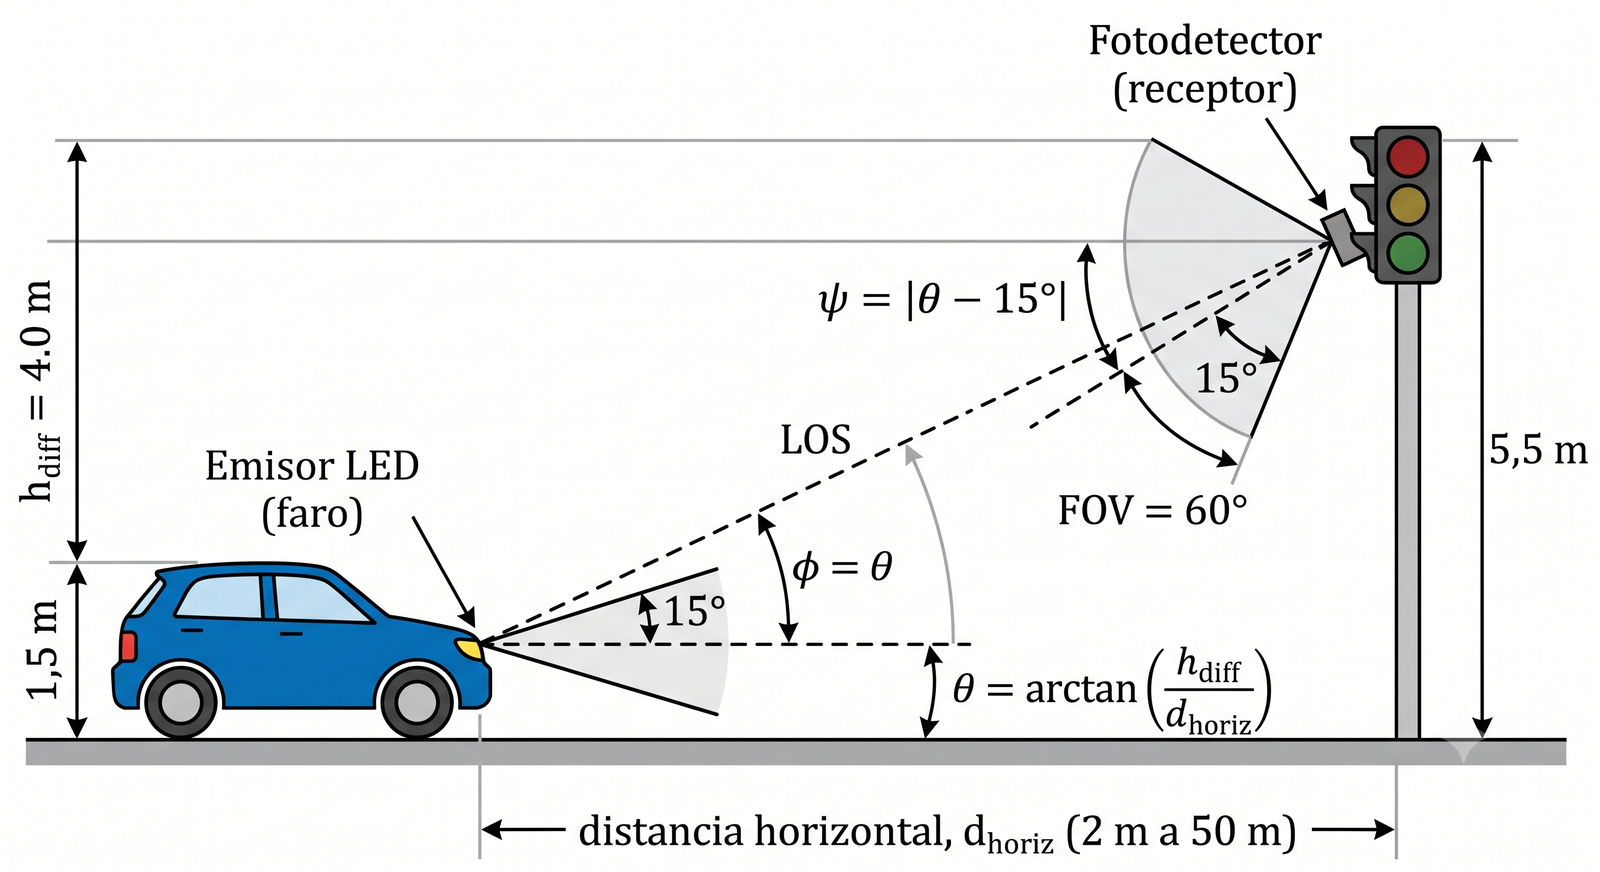
\includegraphics[width=0.85\textwidth]{Diagrama V2I.png}
	\caption{Diagrama esquemático de la geometría del enlace óptico vehicular V2I (uplink) con emisor LED inclinado $15^\circ$ y fotodetector horizontal en la RSU. Se muestran los ángulos $\phi$, $\psi$ y la distancia tridimensional $d$ en función de la posición horizontal $x$ del vehículo.}
	\label{fig:diagrama_v2i}
\end{figure}

En enlaces de línea de vista (LOS, \textit{Line-of-Sight}), donde existe una trayectoria directa y libre de obstáculos entre el emisor y el detector, la ganancia de canal $H(0)$ se calcula matemáticamente mediante el modelo de radiación Lambertiano \cite{ghassemlooy2019optical}:
\begin{equation}
	H(0) = \begin{cases}
		\frac{(m + 1) A_r}{2 \pi d^2} \cos^m(\phi) T_s(\psi) g(\psi) \cos(\psi), & 0 \le \psi \le \Psi_c \\
		0, & \psi > \Psi_c
	\end{cases}
	\label{eq:ganancia_dc}
\end{equation}
donde cada una de las variables físicas interviene en la atenuación de la señal de la siguiente manera:
\begin{itemize}
	\item $d$: es la distancia física tridimensional (en metros) entre la RSU y la Unidad a Bordo (OBU). Debido a la ley del inverso del cuadrado, la potencia óptica recibida decrece cuadráticamente con el aumento de la distancia, constituyendo el factor dominante de pérdida.
	\item $A_r$: es el área de detección física del fotodiodo del receptor (en $\text{m}^2$). Un área mayor capta más potencia óptica, pero incrementa la capacitancia de la unión del semiconductor, restringiendo el ancho de banda efectivo.
	\item $\phi$: es el ángulo de irradiancia del haz emitido por el LED con respecto a la normal del plano de emisión del transmisor.
	\item $\psi$: es el ángulo de incidencia de los fotones con respecto a la normal de la superficie activa del fotodetector.
	\item $\cos(\psi)$: representa el factor de inclinación del receptor. A medida que el ángulo de incidencia se aleja de la normal, el área de captación efectiva disminuye en función de la proyección del coseno, de acuerdo con la ley de Lambert.
	\item $T_s(\psi)$: es la ganancia del filtro óptico pasabanda colocado delante del receptor, cuya función es bloquear la radiación solar y lumínica ambiental fuera de la longitud de onda de interés para mitigar el ruido de disparo.
	\item $g(\psi)$: es la ganancia del concentrador óptico de luz (lente no formadora de imagen), la cual incrementa de forma pasiva la potencia lumínica concentrándola en la pequeña área del fotodiodo. Esta propiedad depende del ángulo de incidencia y se define \cite{ghassemlooy2019optical} como:
	\begin{equation}
		g(\psi) = \frac{n^2}{\sin^2(\Psi_c)}
		\label{eq:ganancia_concentrador}
	\end{equation}
	donde $n$ representa el índice de refracción del material de la lente y $\Psi_c$ representa el semiángulo del campo de visión (FOV) del receptor. Si los fotones inciden en un ángulo que supera este límite ($\psi > \Psi_c$), la ganancia se anula por completo, proporcionando una selectividad espacial natural.
	\item $m$: es el orden de emisión de Lambert, que caracteriza la directividad angular del haz del LED. Este coeficiente se relaciona de forma unívoca con el semiángulo de potencia media del emisor $\theta_{1/2}$ a través de la expresión:
	\begin{equation}
		m = \frac{- \ln(2)}{\ln(\cos(\theta_{1/2}))}
		\label{eq:orden_lambert}
	\end{equation}
	Un valor bajo de $m$ representa un haz disperso e isotrópico (cobertura amplia para iluminación), mientras que un orden elevado concentra el flujo lumínico en un haz colimado y estrecho, incrementando la densidad de potencia a costa de requerir una alineación geométrica más precisa.
\end{itemize}

En escenarios exteriores, a la pérdida geométrica descrita por $H(0)$ se le adiciona la atenuación atmosférica provocada por los fenómenos de dispersión y absorción causados por los aerosoles y partículas de agua suspendidas en el aire. La potencia óptica instantánea recibida a través de un canal ruidoso y atenuado por el clima se modela aplicando la ley de Beer-Lambert \cite{ghassemlooy2019optical}:
\begin{equation}
	P_{\text{rx\_optical}}(t) = H(0) e^{-\beta d} P_{\text{opt}}(t)
	\label{eq:beer_lambert_theory}
\end{equation}
donde $\beta$ es el coeficiente de extinción atmosférica del medio en $\text{m}^{-1}$ y $d$ es la distancia de propagación, con el significado detallado de cada término a continuación:
\begin{itemize}
\item $H(0)$: ganancia DC del canal óptico LOS, calculada mediante la ecuación Lambertiana (Ec.~\ref{eq:ganancia_dc}). Cuantifica la atenuación geométrica pura del enlace directo a la distancia $d$.
\item $e^{-\beta d}$: factor de transmitancia atmosférica derivado de la ley de Beer-Lambert. Representa la fracción de potencia óptica que llega al receptor después de atravesar una columna de aire de longitud $d$ con coeficiente de extinción $\beta$. Para $\beta = 0$ (noche despejada) el factor es 1 y no hay atenuación adicional; para $\beta = 0.15\text{ m}^{-1}$ (neblina) y $d = 10\text{ m}$ el factor baja a $e^{-1.5} \approx 0.22$, lo que representa una pérdida de 6.6~dB.
\item $\beta$: coeficiente de extinción atmosférica en $\text{m}^{-1}$. Suma la contribución de la dispersión (\textit{scattering}) y la absorción molecular. Sus valores por escenario se detallan en la Tabla~\ref{tab:escenarios_clima}.
\item $d$: distancia de propagación en metros. Coincide con la variable $d$ de la Ec.~\ref{eq:ganancia_dc} y es el parámetro de barrido principal en las simulaciones Monte Carlo (rango: 1~m a 50~m).
\item $P_{\text{opt}}(t)$: potencia óptica emitida por el LED en vatios, salida de la Ec.~\ref{eq:p_opt_conv}.
\item $P_{\text{rx\_optical}}(t)$: potencia óptica promedio recibida en el fotodiodo en vatios. Al ser convertida por la responsividad $R$, origina la fotocorriente $i_{\text{rx}}(t) = R \cdot P_{\text{rx\_optical}}(t)$.
\end{itemize}

Adicionalmente, el enlace en exteriores se encuentra sometido a perturbaciones aleatorias de ruido. La corriente de ruido total en el fotodetector se modela mediante un proceso gaussiano aditivo de media cero con varianza total dada por:
\begin{equation}
\sigma^2_{\text{total}} = \sigma^2_{\text{shot}} + \sigma^2_{\text{thermal}}
\label{eq:noise_total}
\end{equation}
donde los términos constitutivos representan la varianza del ruido térmico $\sigma^2_{\text{thermal}}$ (fijada en $10^{-16}\text{~A}^2$, correspondiente al ruido de Johnson-Nyquist de un amplificador de transimpedancia a temperatura ambiente de $300\text{~K}$) y la varianza del ruido de disparo $\sigma^2_{\text{shot}}$ inducido por la luz solar de fondo. La potencia de este ruido de disparo se modela de acuerdo con la relación:
\begin{equation}
\sigma^2_{\text{shot}} = 2 \cdot q \cdot R \cdot E_{\text{sol}} \cdot A_r \cdot g(\psi) \cdot I_2 \cdot B
\label{eq:shot_noise_theory}
\end{equation}
En esta expresión, la variable $q$ define la carga elemental del electrón ($1.602 \times 10^{-19}\text{~C}$), mientras que $R$ introduce el impacto de la responsividad del fotodiodo ($0.6\text{~A/W}$), la cual traduce la irradiancia de fondo en fotocorriente de ruido. La potencia de la radiación solar incidente tras el filtrado óptico del 99.7\% queda determinada por $E_{\text{sol}}$, cuyos valores para los distintos escenarios se detallan en la Tabla~\ref{tab:escenarios_clima}. Por su parte, la recolección geométrica de fotones depende del área activa del fotodetector $A_r$ ($10^{-4}\text{~m}^2$) y de la ganancia del concentrador óptico $g(\psi)$, cuyo valor de diseño es $9$ de acuerdo con la Ec.~\ref{eq:ganancia_concentrador}. Finalmente, la dispersión espectral se rige por el factor de ancho de banda de ruido $I_2$ ($0.562$) y el ancho de banda efectivo del receptor $B$ ($40\text{~MHz}$), que equivale a la mitad de la frecuencia de muestreo de la simulación.

Para cuantificar la calidad del enlace óptico antes del procesamiento en banda base y tras la remoción de la componente continua en el bloque DC~Block, se calcula la SNR instantánea de la señal recibida mediante la relación:
\begin{equation}
\text{SNR} = \frac{\text{Var}\left( R \cdot H(0) e^{-\beta d} s_{\text{clean}}(t) \right)}{\sigma^2_{\text{shot}} + \sigma^2_{\text{thermal}}}
\label{eq:snr_theory}
\end{equation}

La relación matemática expresada en la Ec.~\ref{eq:snr_theory} queda gobernada en el numerador por la potencia útil de la señal, calculada mediante la varianza empírica $\text{Var}(\cdot)$ de la componente de corriente alterna útil de datos en el receptor. Esta señal alterna proviene del producto de la responsividad del fotodiodo $R$, la ganancia DC del canal óptico $H(0)$, el decaimiento atmosférico exponencial de Beer-Lambert $e^{-\beta d}$ y la señal de corriente intermedia unipolar transmitida $s_{\text{clean}}(t)$ tras aislar el bias DC. El denominador introduce el efecto degradante de la potencia de ruido total mediante la suma de la varianza del ruido de disparo $\sigma^2_{\text{shot}}$ y del ruido térmico $\sigma^2_{\text{thermal}}$ (Ec.~\ref{eq:noise_total}), lo que determina la relación de amplitudes antes de la demodulación digital. Para su registro y conversión a decibelios en el script Monte Carlo, se aplica la relación logarítmica clásica $\text{SNR}_{\text{dB}} = 10 \log_{10}(\text{SNR})$.



Para evaluar de forma realista la comunicación V2I bajo diferentes estados del clima y niveles de ruido, se definen cuatro escenarios de simulación parametrizados mediante la irradiancia solar de fondo $E_{\text{sol}}$ y el coeficiente de extinción $\beta$. Estos valores se resumen en la Tabla \ref{tab:escenarios_clima}.

\begin{table}[htbp]
	\centering
	\caption{Parámetros Físicos de los Escenarios Meteorológicos de Simulación.}
	\label{tab:escenarios_clima}
	\begin{tabular}{|p{3cm}|p{2.2cm}|p{2.2cm}|p{7.1cm}|}
		\hline
		\textbf{Escenario} & \textbf{Irrad. Solar Efec.} $E_{\text{sol}}$ & \textbf{Coef. Extinción} $\beta$ & \textbf{Criterio y Limitación Física (Filtro del 99.7\%)} \\ \hline
		Noche Despejada (Ideal) & $0\text{ W/m}^2$ & $0.0\text{ m}^{-1}$ & Canal óptico ideal sin atenuación atmosférica. Ruido limitado por el ruido térmico.\\ \hline
		Día Soleado (Ruido Solar) & $0.5\text{ W/m}^2$ & $0.0\text{ m}^{-1}$ & Ruido de disparo solar máximo ($E_{\text{sol, brut}} = 150\text{ W/m}^2$ atenuado en 99.7\% por filtro selectivo).\\ \hline
		Lluvia Moderada & $0.2\text{ W/m}^2$ & $0.05\text{ m}^{-1}$ & Cielo nublado ($E_{\text{sol, brut}} = 50\text{ W/m}^2$ atenuado). Dispersión geométrica por gotas de lluvia.\\ \hline
		Neblina Moderada & $0.1\text{ W/m}^2$ & $0.15\text{ m}^{-1}$ & Mayor pérdida. Visibilidad corta ($\approx 100\text{ m}$ con sol atenuado). Dispersión Mie extrema.\\ \hline
	\end{tabular}
\end{table}

La selección y calibración de estos parámetros se justifica mediante la literatura científica consolidada en el área de comunicaciones ópticas vehiculares. Los valores de irradiancia solar de fondo, que modelan el peor caso de exposición solar en exteriores, se fundamentan en las mediciones del espectro de luz natural donde se demuestra la eficacia del filtrado óptico del 99.7\% en el fotodetector para reducir la corriente de disparo a niveles estables \cite{ghassemlooy2019optical}. Por otro lado, los coeficientes de extinción atmosférica ($\beta = 0.05\text{ m}^{-1}$ para lluvia moderada y $\beta = 0.15\text{ m}^{-1}$ para neblina moderada) se basan en el modelado del decaimiento óptico y de la visibilidad horizontal en carreteras \cite{uysal2015vlc}, garantizando la precisión del simulador frente a escenarios meteorológicos urbanos reales.

Finalmente, es fundamental delimitar el modelo respecto a la geometría de propagación. Los canales en comunicaciones ópticas inalámbricas se clasifican en enlaces de línea de vista (LOS) y enlaces de no línea de vista (NLOS), los cuales dependen de las reflexiones secundarias de la luz sobre las superficies circundantes. Para las simulaciones de esta tesis se ha seleccionado un \textbf{canal óptico estrictamente del tipo LOS}, decisión que se justifica bajo tres factores de diseño:
\begin{enumerate}
	\item \textbf{Geometría del enlace vehicular (V2I):} En la comunicación vehículo a infraestructura, los emisores ópticos instalados en semáforos o luminarias están elevados y alineados de forma directa con los receptores ópticos montados en los vehículos, garantizando un trayecto despejado.
	\item \textbf{Atenuación severa por reflexión (NLOS):} En entornos exteriores, las superficies como el asfalto poseen coeficientes de reflectancia bajos (típicamente del 5\% al 10\%). Una señal reflejada en la carretera sufre atenuaciones de entre 20~dB y 30~dB en comparación con el rayo directo, provocando que las componentes reflejadas aporten una potencia insignificante que resulta enmascarada por el ruido de disparo solar.
	\item \textbf{Despreciable dispersión temporal (\textit{Delay Spread}):} Debido a que la velocidad de la luz es extremadamente alta y las distancias en carreteras urbanas son de corto a medio alcance (menores a 50~metros), las componentes reflejadas llegan con retrasos temporales que causan un esparcimiento del retardo despreciable para las tasas de transmisión estándar del protocolo IEEE 802.11bb, prescindiendo de la necesidad de incorporar un ecualizador multitrayecto complejo en el receptor.
\end{enumerate}
Por eso, el uso de un modelo de canal estrictamente LOS permite modelar con rigor matemático el comportamiento real de la atenuación de potencia y el cálculo de la relación señal a ruido (SNR), manteniendo una excelente eficiencia computacional sin perder precisión experimental.

\subsubsection{Métricas de evaluación del rendimiento de la capa física}
Para evaluar la calidad del enlace y la robustez del sistema de comunicaciones ópticas vehiculares, se definen dos métricas fundamentales de la capa física: la Tasa de Error de Bit (BER, \textit{Bit Error Rate}) y la velocidad de transmisión efectiva (\textit{Throughput}) \cite{ghassemlooy2019optical}.

La Tasa de Error de Bit (BER) se calcula estadísticamente dividiendo el número de bits erróneos detectados en la salida del decodificador de Viterbi entre la cantidad total de bits de información útiles de prueba transmitidos:
\begin{equation}
	\text{BER} = \frac{N_{\text{errores}}}{N_{\text{total}}}
	\label{eq:ber}
\end{equation}
donde cada término representa lo siguiente:
\begin{itemize}
	\item $N_{\text{errores}}$: número total de bits decodificados de manera errónea en el receptor (cuando un bit originalmente transmitido como 0 es interpretado como 1, o viceversa).
	\item $N_{\text{total}}$: cantidad total de bits de información útil transmitidos en el bloque o trama de simulación.
\end{itemize}

Por su parte, el \textit{Throughput} (o tasa de transmisión efectiva) en Mbps se define como la velocidad neta de transferencia de información útil una vez descontados los bits erróneos de la velocidad bruta de transmisión nominal de la capa física \cite{ghassemlooy2019optical, elgala2011indoor}:
\begin{equation}
	\text{Throughput} = R_{\text{raw}} \cdot (1 - \text{BER})
	\label{eq:throughput}
\end{equation}
donde cada término cumple el siguiente rol en el cálculo:
\begin{itemize}
	\item $R_{\text{raw}}$: velocidad de transmisión física bruta en Mbps, calculada teóricamente a partir del esquema de modulación, la tasa de codificación y la duración del símbolo OFDM correspondientes al MCS seleccionado (según la Ec.~\ref{eq:phy_rate_calc}).
	\item $\text{BER}$: Tasa de Error de Bit instantánea (según la Ec.~\ref{eq:ber}) medida en el punto de operación.
\end{itemize}


